\section{Insertion Sort}
\begin{enumerate}
    \item Si memorizza l'elemento $A[k]$ da sistemare in una variabile $x$
    \item Si ispeziona la porzione di array $A[0..k-1]$ {\emph{da destra verso sinistra}},
    spostando avanti di una posizione ogni elemento maggiore di $x$, in modo da "fare posto"
    all'elemento da inserire
    \item Individuata la posizione in cui inserire $x$ (quindi quando si 
    raggiunge un elemento che non è maggiore di $x$ o quando si è ispezionata
    tutta la porzione iniziale di array), si inserisce $x$ (gli elementi successivi sono già stati 
    spostati durante il passo 3)
\end{enumerate}

\begin{figure}[h]
    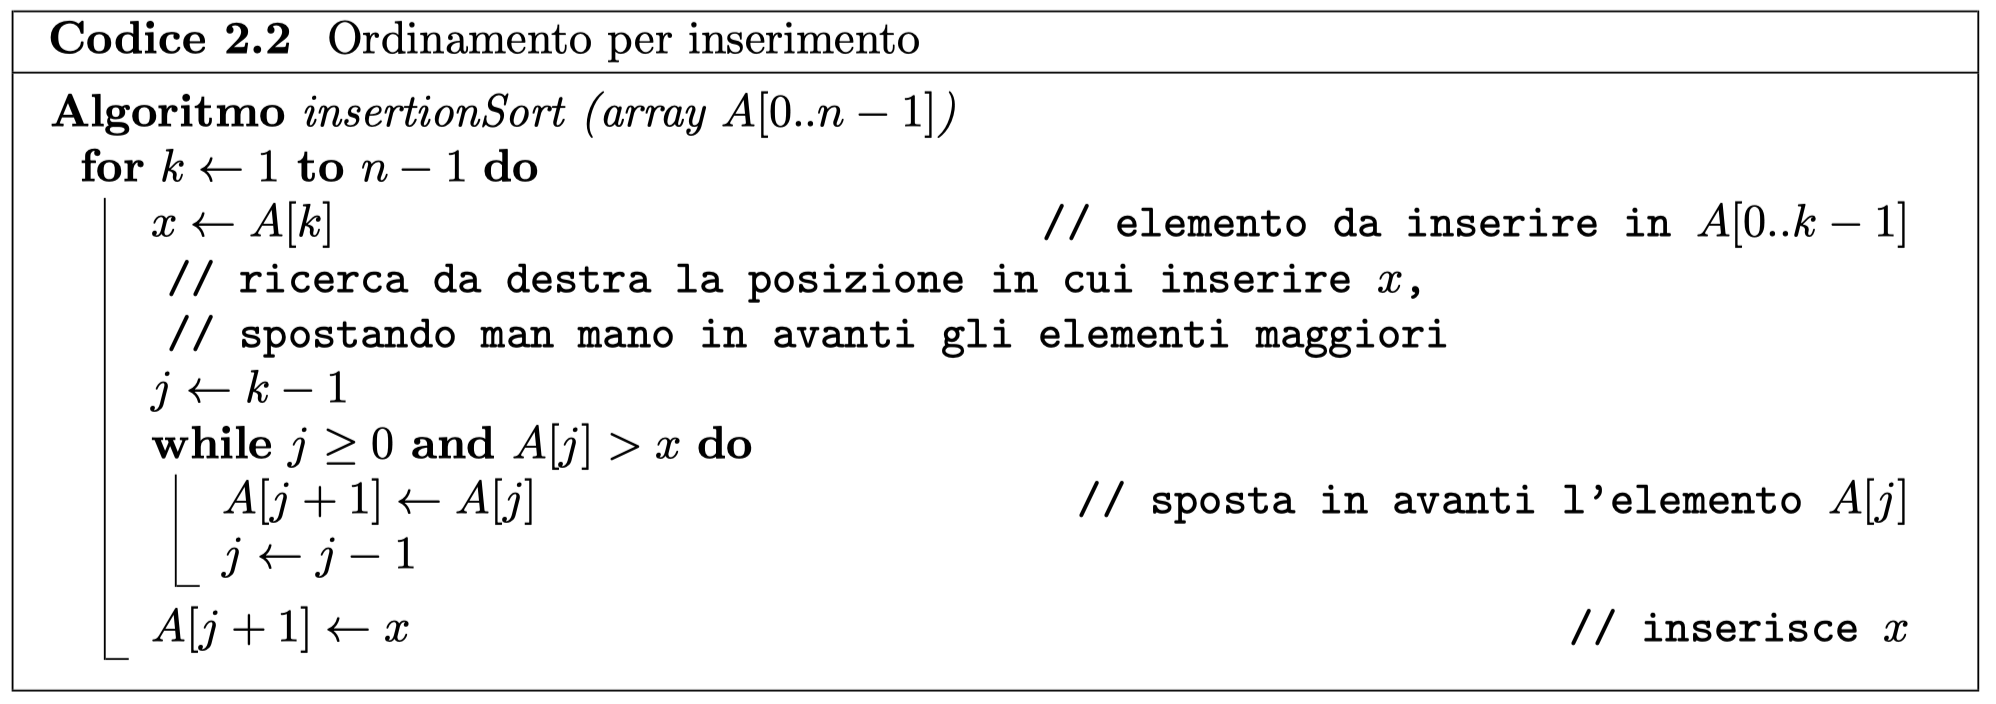
\includegraphics[width=\textwidth]{insertionsort.png}
\end{figure}

\subsubsection*{Numero di confronti}
Nel caso peggiore ogni elemento dell'array viene confrontato con ogni altro
elemento dell'array. Pertanto vengono effettuati $\frac{n(n-1)}{2} = \Theta(n^2)$
confronti. Il caso peggiore si verifica nel caso in cui l'array sia ordinato al 
contrario, mentre nel caso migliore, ovvero quello in cui l'array è già ordinato,
vengono effettuati $n - 1$ confronti.

\subsubsection*{Spazio}
L'algoritmo, oltre all'array da ordinare, utilizza un numero costante di variabili.
Pertanto la quantità di spazio aggiuntivo è costante.
\clearpage